\documentclass[a4wide,10pt]{article}
%\usepackage{a4wide}
\usepackage[applemac,utf8]{inputenc}
\usepackage[danish]{babel}
\usepackage[T1]{fontenc}
\usepackage{pdfsync}
\usepackage{amsmath,amssymb,amsfonts} 
\usepackage[pdftex]{graphicx}
\usepackage{wrapfig}
\usepackage{color}
\usepackage[small,bf]{caption}

\begin{document}
\title{DSB Portfolio 2}
\author{Nis Sarup}
\date{\today}
\maketitle

\newpage

	\section{Fourier Transform method} % (fold)
	\label{sec:fourier_transform_method}
		Mathematica formulas:
		\begin{eqnarray}
			t &=& 67; \nonumber \\
			m &=& \frac{t-1}{2}; \nonumber \\
			cH &:=& \frac{2\pi 1800}{8000}; \nonumber \\
			cL &:=& \frac{2\pi 800}{8000}; \nonumber \\
			h[0] &:=& \frac{cH-cL}{\pi}; \nonumber \\
			h[n_] &:=& \frac{Sin[cH \cdot n]}{n\cdot \pi} - \frac{Sin[cL \cdot n]}{n\cdot \pi}; \nonumber \\
		\end{eqnarray}
		I get the results h[n] with n ranging from $-m$ to $m$:
		\begin{equation}
			Table[h[i], {i, -m, m, 1}]
		\end{equation}
		This gives a large table of values which I copy into the MathLab program (Program 7.1 for example 7.3 in the book) and get the following graph:
		\begin{figure}[htbp]
			\centering
				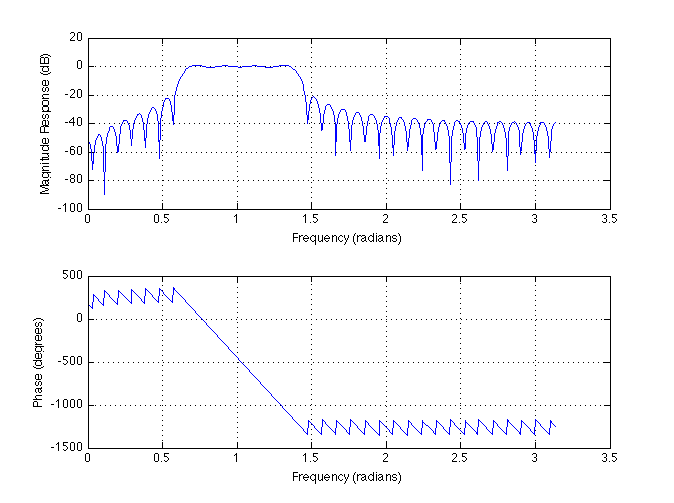
\includegraphics[width=9cm]{images/opgave_1.png}
			\caption{Fourier Transform method: Magnitude response and Phase.}
			\label{fig:images_opgave_1}
		\end{figure}
	% section fourier_transform_method (end)
	
	\newpage
	
	\section{Window Method} % (fold)
	\label{sec:window_method}
		
	% section window_method (end)
	
\end{document}